\documentclass[12pt]{article}
\usepackage{graphicx}
\usepackage{hyperref}
\usepackage{setspace}
\usepackage{caption}
\usepackage{geometry}
\usepackage{float}
\geometry{margin=1in}
\setstretch{1.25}

\title{What If St. Paul Made Vacant Landowners Pay for the Budget Shortfall?}
\author{Matthew Hockert}
\date{\today}

\begin{document}
\maketitle

A few weeks ago I was reading the Axios Twin Cities newsletter and its reporting on the proposed budget from St.Paul Mayor Melvin Carter that he argues avoids layoffs of city workers but raises the property tax levy by 5.3\%. The plan comes as the city faces a \$23 million deficit.  

Property taxes make up almost half (46\%) of St. Paul's \href{https://www.stpaul.gov/sites/default/files/2024-02/2024%20City%20of%20Saint%20Paul%20Adopted%20Operating%20Budget.pdf}{general fund} in 2024. Given it's a significant source of funding and a key instrument in funding itself the city can make adjustments by levying higher taxes to make up for the shortfall. However, St. Paul can only raise property taxes uniformly across property classes, which means everyone pays more, regardless of whether their property is sitting vacant or fully developed. Cities like St. Paul don’t have the authority to vary tax rates based on land use, those classifications are set by the state legislature.  

But St. Paul can adjust certain fees, including the one for vacant buildings, which got me thinking:  

\begin{quote}
What if, instead of raising everyone’s property taxes, St. Paul raised the fees on vacant lots to make up the shortfall?
\end{quote}

\section*{Why It’s Interesting}

This post is purely a hypothetical scenario and an exercise for me as an economist. It is not meant as a formal fiscal policy proposal, but actually to highlight how fee structures, rules on local governance, and how changes in these two can influence behavior. Under Minnesota law the distinction between taxes and fees is significant and ultimately shapes who bears the costs of fiscal shortfalls.

As highlighted above, property taxes are a significant source of general fund revenue and can be used broadly to support the operations of a city. By contrast, fees are much more constrained under the law: they must be tied to the cost of providing a specific service or regulating an activity. For example, a sewer fee can only fund wastewater infrastructure, and a vacant building registration fee can only support code enforcement or maintenance associated with those properties.

Therefore, St. Paul could not legally use higher vacant property fees to make up for the property tax levy increase without legislative action. However, this blog is for fun but may also serve to show how fees can alter the incentives on underutilized land. This approach could, in theory, encourage redevelopment and reduce the number of idle parcels, strengthening the long-run tax base while minimizing impacts on homeowners. (Yes this is essentially a Land Value Tax (LVT) targeting only vacant parcels).


\section*{Methods}

All data and analysis were performed in R and you can find the code in my \href{https://github.com/yourusername/your-repo}{GitHub repository}. The workflow consisted of two main stages:

\begin{enumerate}

    \item Vacancy classification. Parcels were identified as vacant if their DWELL\_TYPE field included the terms ``VACANT'' or ``UNIMPROVED,'' and both EMV\_BLDG == 0 and NUM\_UNITS == 0. A binary indicator variable, vacant\_strict, was assigned to flag these parcels. Parcels associated with redevelopment projects (e.g., ``FORD LOT'' or ``HIGHLAND BRIDGE ROWHOMES'') were excluded because we are in 2025 when I write this and some of these parcels have been developed on. 

    \item Fiscal simulation. The city’s total levy (city\_levy\_est) was estimated from parcel tax capacity and an assumed city tax rate (city\_rate = 0.497). The city tax rate comes from dividing the levy by the total tax capacity, which you can find \href{https://www.stpaul.gov/sites/default/files/2024-08/Major%20City%20General%20Fund%20Revenues%202025%20Proposed.pdf}{here}. A hypothetical shortfall of 5.3\% was calculated and divided by the number of vacant parcels to estimate the required annual vacant parcel fee needed to offset the shortfall. I then perform a sensitivity analysis where I varied the vacancy miscount rate from 50\% to 100\%, computing required fees under different assumptions of parcel coverage. I did this because I some varying numbers in the media about how many parcels are considered vacant.
\end{enumerate}

\section*{Vacant Building Regulations}

According to the \href{https://www.stpaul.gov/departments/safety-inspections/rent-buy-sell-property/vacant-buildings/vacant-building-program}{City of Saint Paul}, property owners must register vacant or unoccupied buildings with the Department of Safety and Inspections if a building is unoccupied and meets any of the following conditions:

\begin{itemize}
    \item The building is unsecured.
    \item The building is secured by other than normal means.
    \item The building is considered a dangerous structure.
    \item The building has been condemned.
    \item The building has multiple housing or Building Code violations.
    \item The building is condemned and illegally occupied.
    \item The building has been unoccupied for more than one year and the Enforcement Officer has issued an order to correct nuisance conditions.
\end{itemize}


Under the Saint Paul Legislative Code, \href{https://library.municode.com/mn/st._paul/codes/code_of_ordinances?nodeId=PTIILECO_TITVIBUHO_CH43VABU_S43.03VABURE}{Section 43.02}, owners of registered vacant buildings are required to pay an annual registration fee. The fee is designed to recover the city’s administrative and enforcement costs associated with monitoring these properties. In this post, I am creating a hypothetical world where we can use these fees to offset the budgetary shortfall and not have to use the fees in the traditional way. The fee schedule is structured by category as follows:

\begin{itemize}
    \item Category I: \$2,705 per year.
    \item Category II: \$2,705 in the first year and \$5,410 per year thereafter.
    \item Category III: \$5,410 per year.
\end{itemize}

\section*{Crunching the Numbers}

I pulled St. Paul’s 2024 parcel data, given my methods above is roughly 1,339 vacant parcels. \\

\begin{figure}[H]
    \centering
    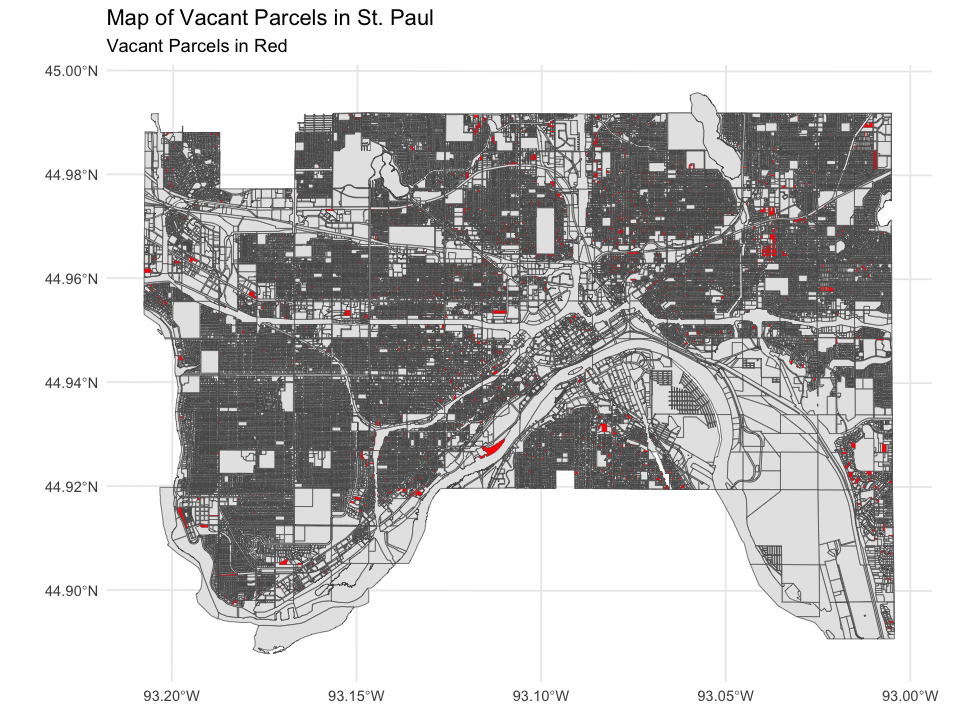
\includegraphics[width=0.9\linewidth]{Map of Vacant Parcels in St. Paul.png}
    \caption{St. Paul's vacant parcels mapped}
\end{figure}

The current minimum vacant building fee is about \$2,705 per year. To cover the city’s shortfall without touching property taxes, those vacant parcels would need to carry the load through higher fees. Here’s what that looks like:

\begin{figure}[H]
    \centering
    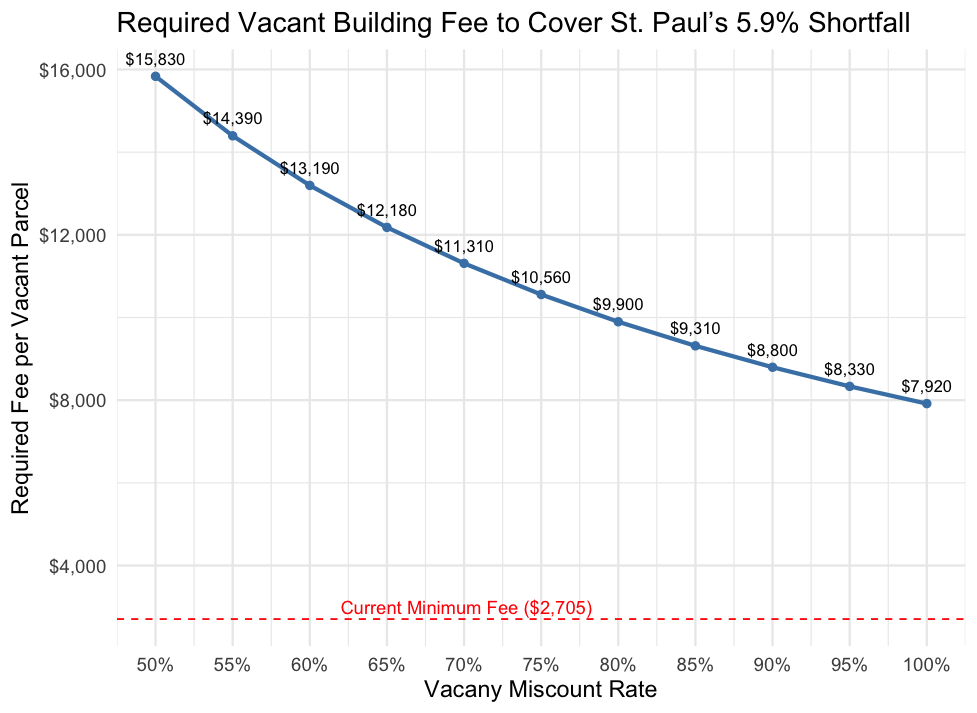
\includegraphics[width=0.9\linewidth]{st_paul_vacant_building_fee_graph.png}
    \caption{Required Vacant Building Fee to Cover St. Paul’s 5.9\% Shortfall}
\end{figure}

The chart shows how high the vacant lot fee would need to be, depending on how accurate my parcel count is.  

\begin{itemize}
    \item If I perfectly counted all 1,339 parcels (100\% on the right), each lot would need to pay about \$7,490 annually — nearly 3x the minimum fee.
    \item If I over counted by half (only about 700 real vacant parcels), the required fee would jump to nearly \$16,000 per parcel — almost 6x higher than the minimum.
\end{itemize}

\section*{Big Picture}

Taxes and inefficient land use effects all residents of the city. By taxing vacancy instead of productive land use, cities could encourage denser development and strengthen their long-term tax base, without overburdening homeowners and renters. This is in essence a land value tax. However, in this hypothetical the most efficient keep the their taxes the same and not reduced whereas in LVT the distribution would hypothetically shift away from the most productive parcels to the least heightening the development pressure. For now, until cities can legally be more creative with their funding, St. Paul’s budget reality means higher property taxes. 

\end{document}